\documentclass[../main.tex]{subfiles}

\begin{document}

\chapter{代码结构}

正文在这里

\textbf{粗体}

\uline{下划线}

xxx

%\setlength{\columnsep}{0.7cm}
\begin{wrapfigure}{r}{0.4\linewidth}
%\vspace{-0.3cm}
\centering
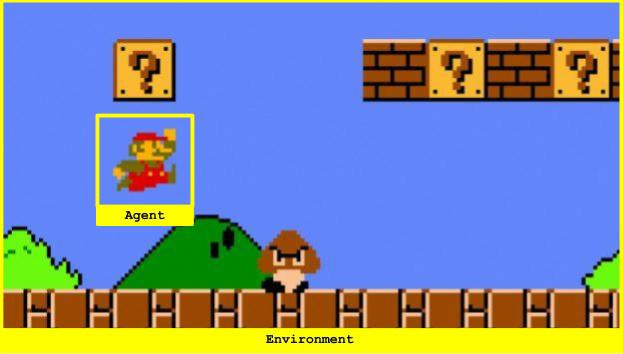
\includegraphics[width=0.4\textwidth]{figures/agentenv.png}
%\caption{Пример среды с двумя действиями.}
%\label{fig:env}
%\vspace{-2.6cm}
\end{wrapfigure}


\end{document}